\documentclass[11pt,border=4pt]{standalone}
\usepackage{amsmath,amssymb,bm,mathtools}
\usepackage[fontset=fandol]{ctex}
\usepackage{tikz}
\usetikzlibrary{arrows.meta,calc,patterns,angles,quotes,decorations.markings,decorations.pathmorphing}
\newcommand{\dd}{\mathop{}\!\mathrm d}
\newcommand{\e}{\mathrm e}
\tikzset{axis/.style={->,>=Stealth,line width=.45pt},world/.style={line width=.8pt},flow/.style={->,>=Stealth,line width=.7pt},ray/.style={->,>=Stealth,line width=.7pt},guide/.style={dashed,line width=.35pt},aux/.style={dashed,line width=.35pt},dim/.style={<->,>=Stealth,line width=.35pt},every node/.style={font=\small},force/.style={->,>=Stealth,very thick},gas/.style={fill=blue!7}}
\begin{document}
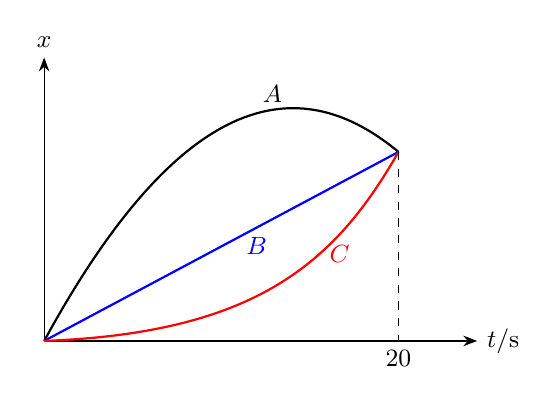
\begin{tikzpicture}\draw[axis](0,0)--(5.5,0)node[right]{$t/\mathrm s$};\draw[axis](0,0)--(0,3.6)node[above]{$x$};\draw[world](0,0)..controls(1.8,3.3)and(3.3,3.4)..(4.5,2.4);\node[above]at(2.9,2.9){$A$};\draw[blue,world](0,0)--(4.5,2.4);\node[blue,below]at(2.7,1.44){$B$};\draw[red,world](0,0)..controls(2.7,.1)and(3.7,1)..(4.5,2.4);\node[red,right]at(3.5,1.1){$C$};\draw[guide](4.5,2.4)--(4.5,0);\node[below]at(4.5,0){$20$};\end{tikzpicture}
\end{document}
